\section{Summaries}

Summaries are used to represent and describe the information contained in datasets. They csan be graphical summaries, which visually represent the data, or numerical summaries, which give a description of the data in terms of numbers.

\subsection{Graphical summaries}
\paragraph{Empirical CDF} A random variable is completely characterized by its CDF. We can approximate the CDF with the empirical cumulative distribution function, which is defined as
\begin{equation*}
    F_n(x) = \frac{|\{ i : [1,n] | x_i \leq x \}|}{n}
\end{equation*}
where the $x_i$ are the observations in the dataset. The \textbf{Glivenko-Cantelli theorem} states that the empirical CDF converges to the true CDF as $n$ goes to infinity:
\begin{equation*}
    P(\lim_{n \to \infty} \sup_x |F(x) - F_n(x)| = 0) = 1
\end{equation*}
This approximation can be plugged into different formulas to estimate other quantities, such as the mean or the variance.

\paragraph{Bar plots and histograms}
A bar plot is used for discrete data. It provides a frequency count for the values in the dataset, and approximates the PMF (as a consequence of the law of large numbers, as seen in a previous example):
\begin{equation*}
    P(X = a) \approx \frac{|\{ i | x_i = a \}|}{n}
\end{equation*}
A histogram is used for continuous data. It provides frequency counts for ranges of values (instead of individual ones). The support of the random variable is first split into $m$ intervals called \textbf{bins} (which can all have the same width or different widths), and the number of occurrences belonging to each bin is counted and normalized:
\begin{equation*}
    A_i = \frac{|\{ j \in [1,n] |x_j \in B_j\}|}{n} \approx P(X \in B_i)
\end{equation*}
The bins can be plotted as rectangles so that their area is proportional to $A_i$; after fixing their width $b_i$, the height is found as $H_i = A_i / b_i$.

Bin width can be chosen in different ways, producing different results. It is common to choose the same width for all bins, such that, for a total number of bins $m$, the interval corresponding to the $i^{th}$ bin is
\begin{equation*}
    B_i = (r + (i-1)b, r + i*b)
\end{equation*}
where $r$ is the minimum value taken by the random variable, and $b$ is the bin width. The optimal width can be found using \textbf{Mean Integrated Squared Error} (\textbf{MISE}):
\begin{equation*}
    MISE = \E \left [ \int (\hat{f}(t) - f(t))^2 \ dt \right ] = \int \int (\hat{f}(t) - f(t))^2 f(x_1) \ldots f(x_n) \ dt dx_1 \ldots dx_n
\end{equation*}
where $\hat{f}$ is the density estimation of the real PDF $f$. The minimum of the MISE for Normal distributions is represented by \textbf{Scott's normal reference rule}:
\begin{equation*}
    b = 3.49 \cdot s \cdot n^{-1/3}
\end{equation*}
wher $s$ is the sample standard deviation.\\
Other options are:
\begin{itemize}
    \item \textbf{Freedman-Diaconis' choice}:
    \begin{equation*}
        b = 2 \cdot \text{IQR} \cdot n^{-1/3}
    \end{equation*}
    This choice is more robust to outliers than the previous.
    \item \textbf{Variable bin width} (such as logarithmic binning as seen in power-law distributions).
    \item \textbf{Fixing the number of bins, and derivaring the width from it}. Some common strategies are:
    \begin{align*}
        &m = \lceil \frac{\max x_i - \min x_i}{b} \rceil\\
        &m = \lceil \sqrt{n} \rceil\\
        &m = \lceil \log_2 n \rceil + 1 \text{ (Sturges' rule)}
    \end{align*}
    The latter assumes normal distribution for the true density. This distribution can be approximated by a $Bin(n, 0.5)$ distribution, so the absolute frequency of the $i^{th}$ bin is $\binom{m-1}{i}$. The total frequency is $n = \sum_{i=0}^{m-1} \binom{m-1}{i} = 2^{m-1}$, from which $m$ is derived.
\end{itemize}

\paragraph{Kernel density estimation}
A big disadvantage of histograms is that the result strictly depends on the number of bins/bin width chosen to visualize the data. Kernel density estimation is another popular method to summarize distributions which is not as sensitive to the choice of parameters.

The idea behind this method is to mix kernel functions (which can take different forms, see Fig \ref{fig:kernels}) centered in each observation in the dataset. Since data is assumed to be of continuous nature, the presence of a certain value in the dataset also contributes to the density of the values around it. The kernel function models the way this density is distributed around that single observation, and by mixing together all the kernels, the result should be a good approximation of the true density.
\begin{figure}[h]
    \centering
    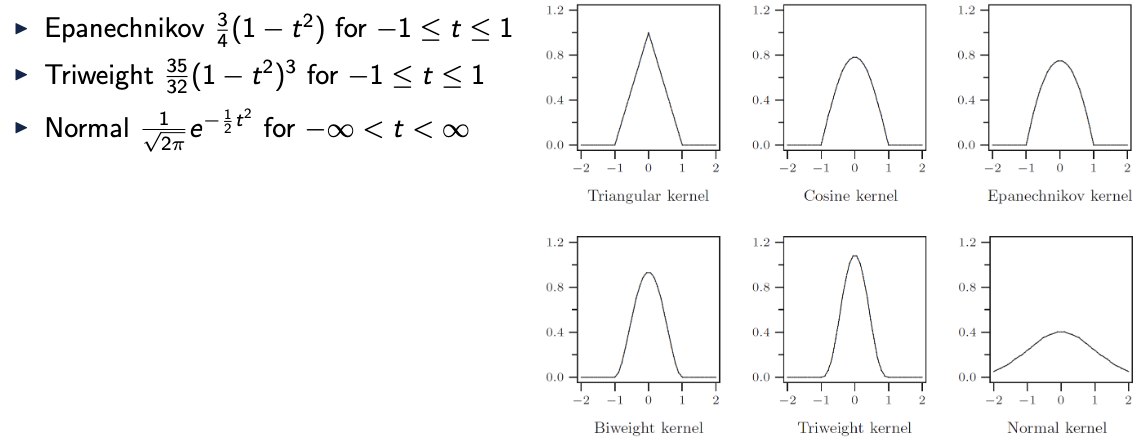
\includegraphics[width=0.8\textwidth]{img/kernels.png}
    \caption{Examples of common kernels used in KDE.}
    \label{fig:kernels}
\end{figure} \\
\boxdefinition{Kernel}{
    A kernel is a function $K : \mathbb{R} \to \mathbb{R}$ such that
    \begin{itemize}
        \item $K$ is a probability density: $K(t) \geq 0$ and $\int_{-\infty}^{\infty} K(t) \ dt = 1$
        \item $K$ is symmetric: $K(-t) = K(t)$
        \item $K(t) = 0$ for $|t| > 1$ (i.e., support is $[-1, 1]$)
    \end{itemize}
}
The last requirement is not strictly necessary, actually; for example, the Normal kernel has unbounded support.

Each kernel function is characterized by a center (the observation), and a \textbf{bandwidth} $h$, which is a scaling factor over the support of the kernel from $[-1, 1]$ to $[-h, h]$. In other words, the badwidth determines how tall-thin or short-wide the kernel is around its center. We can then write
\[
    X \sim K(t) \implies h \cdot X + x_i \sim \frac{1}{h} K \left ( \frac{t - x_i}{h} \right )
\]
because of the change-of-units transformation formulas. The final kernel density estimate is the result of the \textbf{mixture} of all the scaled and shifted kernel densities:
\begin{equation*}
    f_{n,h} (t) = \frac{1}{nh} \sum_{i=1}^n K\left ( \frac{t-x_i}{h}\right )
\end{equation*}
The $1/n$ in the formula is a normalization factor that ensures the density integrates to 1.

The choice of kernel is not critical to the final result; different kernels behave similarly. The key parameter is the bandwidth $h$. Also for KDE, MISE can be used to find the optimal value. Assuming the true density is Normal, the MISE is minimized for
\begin{equation*}
    h = \left (\frac{4}{3} \right )^{1/5} \cdot s \cdot n^{-1/5}
\end{equation*}
For other distributions, the optimal bandwidth can be found using plug-in selectors or cross validation selectors.

Another issue that may arise is when the support of the random variable is bounded. If KDE is used as is, the result will present density event corresponding to values that are not possible. To avoid this, boundary correction techniques are used; some examples are
\begin{itemize}
    \item Kernel truncation and renormalization (forced truncation of the kernel outside the support);
    \item Linear combination kernel;
    \item Beta boundary kernels;
    \item Reflective kernels.
\end{itemize}

\subsection{Numerical summaries}

